\fancyhead[CO]{APPENDIX \thechapter: \leftmark}

\chapter{The Seven-Term System of Francisco Guerrero and Complete Formalization}
\label{AppendixA}

\lettrine[lines=2,slope=-2pt,nindent=2pt]{\textcolor{SchoolColor}{I}}{n the following appendix} is a translation of an article written by Francisco Guerrero Marín in collaboration with mathematician Juan José Morales in Scherzo magazine in 1990.\footnote{\citet{guerrerotopology}} This article introduces both Guerrero's 7-term system, used in the works \textit{Zayin II}, \textit{Rhea}, and \textit{Nur,} as well as his concept of topoligical invariance in formal structures. This very brief summary does not actually analyze any specific works to show the techniques in action, rather the article merely formalizes the two techniques. The topological principle seems to relate to invariant structures across sections such as rhythmic materials, numbers of silences, harmonic materials, and structural elements such as the orchestrational distribution of materials. The mathematical expression in the article is not sufficiently explained but likely refers to the proportional distribution of events, not only in the large scale form, but also within each instrumental line of a given section. Possibly, a first set of reference durations of large sections and subsections is first produced with the Equation \vref{eq:guerrero-proportions}. After this, the proportions of each voice are derived from the proportions of a different voice with the inclusion of some random variation.\footnote{Translator's note: As a result of the use of random values and cross-relationships between voices, it is impossible to reverse-engineer the process of a specific composition without a sketch archive.} In this way, each individual line of the score is in slightly longer or shorter proportion to the others, causing most section transitions to occur over an interpolation period instead of an immediate section change across the whole ensemble as is found in the older pieces, such as \textit{Zayin I}. Due to the low quality of my digital copy of the document, some small characters in the equations are difficult to discern. As a result, it has been sometimes necessary to guess their meaning.\footnote{A digital, full copy of the original magazine issue is freely available from \url{https://scherzo.es/hemeroteca/marzo-1990/}.}

\section{From `Musica Y Tecnologia' of issue 43 of \textit{Scherzo}}

\textbf{Music and Topology}

Zayin II, for string trio, Rhea, for twelve saxophones, and above all Nur, for choir, have been the starting points when establishing a part of the theoretical body that is described later. Part of it was already founded at the time of the composition of both works and the rest was deduced, expanded and inspired by the works themselves. Certain behavioral systems have been codified in order to give them a logical structure that allows their application and development. Since music is a phenomenon of expansion in time, it was thought that topology (expansion in space) could teach us behaviors of mobilities and transformations from a point of view that included partial topologies (for example fractals, chaos) and balance mechanisms that are related to information theories.

\textbf{Brief analysis of Nur}

Let S be the entire work. An element of S is each of the well-defined materials or sound events that compose it, and each of the parts of the work is class-L. Now let the following axioms be:

Axiom 1: If A and B are distinct elements of S, there exists at least one L-class containing A and B.

Axiom 2: If A and B are two distinct elements of S, there is only one L-class that contains A and B.

Axiom 3: Any two L-classes have at least one element of S in common.

Axiom 4: The L-classes are formed by three elements of S.

Thus, for example, for the set S = (A, B, C, D) there is no possibility of applying the axioms without obtaining contradictions.

For the set S = (A, B, C, D, E, F, G) we would obtain the following set of L-classes.

S= (ABC, BDE, DCF, CEG, EFA, FGB, GAD)

In this way, the content of the material of each part of the work is achieved and also defines the general form. The evolution of the material is done attending to a certain types of invariances that develop in a spatiotemporal dimension; space and time are two dimensions to which the same treatment is applied here. These invariances refer, for example, to the conservation of the number of beats (it is the minimum unit of time used: 16th note, 32nd note, etc.), to the maintenance of certain rules of constant proportion, etc., thus achieving an unstable balance that allows for evolution.

If the previous axioms defined the form and related materials, the rules that govern the proportions, both at a general level and instrumental part by part, are given by the following expression:

\begin{equation}
t(A_{i}) = \frac{T}{\displaystyle\sum_{i=1}^{n} m \Delta_{i} \textstyle\sum_{\substack{j=p\\ j \neq i}}^{p+k} t'(A_{j})} t'(A_{i})
\label{eq:rhea}
\end{equation}

Where:

T: Actual duration of the work.

t(A\textsubscript{i}): Duration of section A\textsubscript{i}.

m: Random number.

$\Delta_{i}$: Proportion parameter, dependent on section i.

$t'(A_{i})=m\Delta_{i}\displaystyle\sum_{\substack{j=p\\ j \neq i}}^{p+k} t'(A_{j})$: Time of imaginary distribution.

In this way all the elements are related and the desired formal unity is achieved.

The temporal dimension entails a notion of distance so we will have in reality a metric structure that induces a topology, being able to define other distances than the usual one, thus obtaining different metric topologies. Suppose we have two fragments of the work, $X$ and $Y$ with their corresponding topologies and we will call points of the spaces $X$ and $Y$ infinitesimal musical gestures, that is to say, they develop in a sufficiently small temporal interval (sextuplet 16\textsuperscript{th} note, 64\textsuperscript{th} note, etc.). We can define a function $f$ that takes us points of $X$ to points of $Y$. Such a function is said to be continuous if the points near point $p$ are sent by $f$ to points near $f(p)$ for any point $p$.

Two sections X and Y are said to be homeomorphic or topologically equivalent if there exists a function (one to one correspondence in this case) that sends points of X to points of Y that is continuous and such that the inverse function (the one that takes points from Y to points from X) is also continuous.

% \begin{figure}[H]
%     \centering
%     \includegraphics[width=80mm]{lilypond/graph.png}
%     %\caption{Caption}
%     \label{fig:guerrero-graph}
% \end{figure}

\begin{figure}[H]
\centering
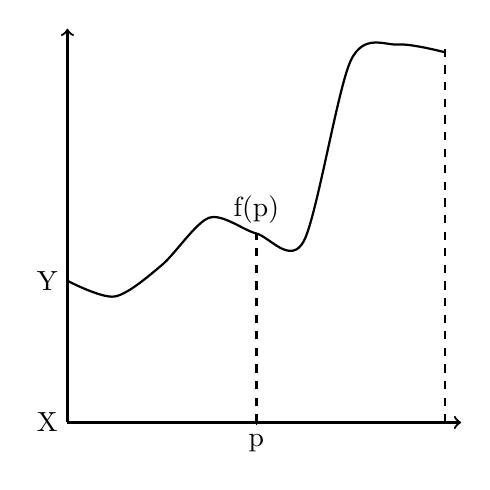
\begin{tikzpicture}
\draw[thick,->] (0,0) -- (5,0) ;
\draw[thick,->] (0,0) -- (0,5) ;
\draw (2.4 cm,1pt) -- (2.4 cm,-1pt) node[anchor=north] {p};
\draw[thick,dashed] (2.4,0) -- (2.4,2.4) node[anchor=south] {f(p)};
\draw[thick,dashed] (4.8,0) -- (4.8,4.8);
\draw [thick] plot [smooth] coordinates {(0,1.8) (0.6,1.6) (1.2,2) (1.8,2.6) (2.4,2.4) (3,2.3) (3.6,4.6) (4.2,4.8) (4.8,4.7)};
\draw (0,1.8) node[anchor=east] {Y};
\draw (0,0) node[anchor=east] {X};
% \foreach \y in {0,1,2,3,4}
%     \draw (1pt,\y cm) -- (-1pt,\y cm) node[anchor=east] {$\y$};
\end{tikzpicture}
    \label{fig:guerrero-graph}
\end{figure}

For example, the vertical projection between the straight line X and the curved line Y is a homeomorphism that intuitively is nothing more than a continuous deformation.

These continuous applications can be used to construct variations of material, since this, when evolving, creates surfaces topologically equivalent to n-toros in two dimensions where n would indicate, for example, the content in silences (the number of holes on the surface), a transformation specific to the material (unisons or its opposite, gliss, etc...).

In addition to these purely sonorous ones, others can be built whose presence is not perceptible, but which in some way direct the musical events. They are related to the abstract content of the work. This is where the use of metrics not related to temporal perception and even topological ones defined without using the notion of distance is most useful. If we define a distance we construct sets formed by elements whose distance to a given one is strictly less than a certain value. The union of all these sets (called open) determines a basis for the topological space.

Without using the notion of distance, a topological space can also be defined. Thus, given a non-empty set $X$ and for each point $p$ of $X$ a non-empty family $B(p)$ of subsets of $X$, it would be said that each family $B(p)$ is a base of open environments of point $p$ if the following properties are verified.

$B_{1}$: If $U$ is an element of $B(p)$ then $p \in U$.\footnote{TN: p is an element of U.}

$B_{2}$: If $U \in$ $B(p)$ and $V \in B(p)$ then there exists $W \in B(p)$ such that $W \not\subset U \cap V$.\footnote{TN: W is not a subset of the intersection of U and V.}

$B_{3}$: If $U \in B(p)$, for each point $q \in U$ there exists a set $V \in B(q)$ such that $V \subset U$.\footnote{TN: V is a subset of U.}

A subset $A$ of $X$ is said to be an open set when in the empty set, or when for each point $t \in A$\footnote{TN: t in A} there is a subset $U \in B(t)$ that is contained in $A$.

It is called the topology $T$ of the set $X,$ determined for the bases of open environments $B(p)$, to the family of open sets of $X$ defined by means of the bases of open environments $B(p)$.

A topological space is compact if each sequence of points has a limit point that belongs to said space. It is connected if it is made of a single piece, that is, if there are no two disjoint open spaces distinct from the vacuum, $V$ and $W$, such that $X=V \cup W$.\footnote{TN: X is the union of V and W}

It is separable (in the sense of Hausdorff)\footnote{TN: Referring to topological separation axioms.} if for every pair of points $p$ and $q$ there exist two disjoint open sets containing $p$ and $q$ respectively. Homeomorphisms preserve all topological properties such as compactness, connectedness, and separability.

Thus, then, we could build a base of open environments from whose expression the general form of the work would result and in such a way that the homeomorphisms between subspaces, whose topology was defined by such base, would control the evolution of local events; They would create rules that as such are constructed to be violated at the moment when an aesthetic choice requires it. In this way, modes of behavior can be created that encompass other destinations (molecular movements, fractalized melodic designs, etc...) but rather replace them and that in no way imply any moral direction. All of this refers to a basis of thought and not to a simple composition setting, thus resulting in empty structures that the musician must fill. It is about seeking order and not a particular order.

\phantom{text} \hfill Juan José Morales and Francisco Guerrero%\footnote{\citet{guerrerotopology}}

\section{Explanation of the Mathematical Expression}

While not every element in equation \ref{eq:rhea} is named and demonstrated, some aspects can be explained. To renotate with some simplifications, the expression could be:

\begin{equation}
X = \frac{T}{S} \cdot Y
\end{equation}

Where X is the duration of a section of the work in a particular voice, T is the total duration of the work, Y is the duration of the same section in a difference voice, and S is the sum of the duration all subsequent sections in a different voice, with some random proportional variation. If all sections and sub-sections of a work are derived from another, a source section must exist. If we take, as a basis, the system described in equation \vref{eq:guerrero-proportions} and the subsequent example proportions, we can try to calculate the proportions of a new voice with the system described in the article above. We begin with a total duration of 240, with section proporitons of 1.8, 2.4, 3.3, 3.6, and 5.4, and calculated section durations of 26.18, 34.9, 48, 52.36, and 78.54. We insert these values into the simplified equation:

\begin{equation}
V_{1}s_{1} = \frac{240}{S} \cdot 26.18
\end{equation}

Where $v1s1$ is voice 1 section 1, and S is the compound summation expression

\begin{equation}
\displaystyle\sum_{i=1}^{n} m \Delta_{i} \textstyle\sum_{\substack{j=p\\ j \neq i}}^{p+k} t'(A_{j})
\end{equation}

In this expression, there is a summation inside of another summation. The lower summation can be written as

\[
[A_{j} + A_{j + 1} + ... + A_{j+k}]
\]

Where the section identified j indications a section other than i, however the authors of the article do not define k. Without an explanation of the value of k, no further calculations are possible. The outer summation can be expressed as

\[
[m \cdot d_{1} \cdot s_{2} + m \cdot d_{2} \cdot s_{3} + ... + m \cdot d_{n} \cdot s_{n+k}]
\]

Where m is a random number, d is the proportion value of section i, and s is the summation of all section durations from j to j+k.

If we take p+k to be the number of subsequent sections, it is possible to calculate all but the final section. For this example, let us imagine that the final duration in our source set is used purely for this calculation purpose and does not represent its own section. Under these conditions we can propose a summation of

\begin{equation}
V_{1}(A_{1}) = \frac{240}{\displaystyle\sum_{i=1}^{4} m \Delta_{i} \textstyle\sum_{\substack{j=2\\ j \neq i}}^{2+k} t'(A_{j})} 26.18
\end{equation}

\subsection{Nested Summations}

i=1, m=0.75, $\Delta$=1.8, and j=2. First we sum all sections in the source durations from 2 until 5. This gives

\[
34.9 + 48 + 52.36 + 78.54 = 213.8
\]

We multiply this value with the others

\[
0.25 \cdot 1.8 \cdot 213.8 = 96.2
\]

We increment i, get a new random value and start again. i=2, m=0.9, $\Delta$=2.4, and j=3.

\[
48 + 52.36 + 78.54 = 178.9
\]

We multiply this value with the others

\[
0.1 \cdot 2.4 \cdot 178.9 = 42.9
\]

We increment i, get a new random value and start again. i=3, m=1.2, $\Delta$=3.3, and j=4.

\[
52.36 + 78.54 = 130.9
\]

We multiply this value with the others

\[
0.3 \cdot 3.3 \cdot 130.9 = 129.6
\]

We increment i one last time, get a new random value and start again. i=4, m=1, $\Delta$=3.6, and j=5.

\[
78.54 + 0 = 78.54
\]

We multiply this value with the others

\[
0.07 \cdot 3.6 \cdot 78.54 = 19.8
\]

We take the sum of these values

\[
96.2 + 42.9 + 129.6 + 19.8 = 288.5
\]

% \subsection{Time of Imaginary Distribution}

% The article says to do this but I chose not to because it's confusing? The article even has a typo there so I'm not sure if I trust it?
% $34.9 + 48 + 52.36 + 78.54 = 213.8$

% $0.045 \cdot 1.8 \cdot 213.8 = 17.32$

\subsection{Final Calculation}

This completes the whole expression. So the source value of 26.18 is recalculated as

\begin{equation}
V_{1}(A_{1}) = \frac{240}{288.5} 26.18 = 21.8
\end{equation}

This process would be repeated for each main section of the work, deriving the first voice from the source values, then deriving subsequent voices from each of the newly calculated voices. This process could conceivably be applied to subsections within a section that is used to denote a statement of more than one material type, perhaps even in the same proportions as the whole work, producing a kind of self-similarity. Note that constraining the range of the random values in this calculation has a significant effect on the resultant duration. Higher random values shorten the duration to a small output value and smaller random numbers give a result closer to the source value. So, a composer could constrain the random values to incredibly small decimals if the source value is intended to be more precise or the values could have a wider range, allowing for a more orchestrationally uncoordinated progression. To reiterate, without Guerrero's sketch materials and without a more thorough explanation of the calculation process in the Scherzo article, it is not possible to know exactly how this formula is intended to be deployed. However, the results illustrated above suggest a possible approach for deriving section durations with an interpretation of the given formula. Through the use of systems like those described above, composers have the ability to generate totally interrelated structures across the duration and instrumentation of a work which is attractive from the project of musical Modernism.\footnote{However the process described above may be incorrect. The inclusion of a random value almost totally negates any usefulness of any of the other parameters. Guerrero could just as easily have multiplied a section's projected duration by any arbitrary fraction near 1 within his own tolerance of variation.}

\section{Bača's Use of Total Formalization}

Trevor Bača's compositions from 2005-2011 use more completely formalized structures than were seen in \textit{Akasha}. What \emph{can} be seen in the compositions from this period is a greater reliance on the slow exposition of material bound to a strict algorithmic pattern. The pieces are quite long, allowing for the playing-out of the strucure underlying the form and material. The segments themselves are longer than would be the norm in later works. While the logic within each work is mostly developed without interference, much effort was taken to iterate the patterns to their ultimate form, resulting in a strikingly rigorous output. The primary aesthetic is that of the phenomenological experience.

\subsection{Po\`eme r\'ecursif (2003/05)}

\begin{quote}
\singlespacing
``Inasmuch as musical form can be equated to a through-time experience of listening for moments of musical change, the formal experience of my earlier music suggests what can understood as a phenomenological, as opposed to narrative, point of departure. \textbf{Po\`eme r\'ecursif}, for sixty-four pieces of percussion, was written in 2005 and recorded by percussionist Brian Archinal in two different mixes on his album \textit{self | space}. The music provides what is an essentially unarticulated experience of form. Tempo is fixed at the beginning of the piece and thousands of attackpoints, all played on unpitched instruments left to the choice of the performer or performers, comprise the seething texture of the music: these provide no shape equivalent to the musical phrase or section. The music ends only at the end of the piece. But the music begins many times, again and again, producing a sense of unending upwelling. Because the materials in \textit{Poème récursif} expose no musical events likely to be construed at the level of narrative -- no sudden stops or starts, no reversals, no enchaining of materials in such a way as to allow for ascriptions of causality -- perception of the music leads instead to an awareness of the act of perception itself. This metaperception is what I intend in invoking the phenomenological in the description the music: recurrent moments when the mind becomes aware of the ways that the mind experiences the music’s currents as phenomena that arise, persist and depart, overlapping in the field of perception. The materials and title of the music point to the recursion that produces these effects: every attackpoint derives from the compositing of two cellular automata over a matrix of 256 columns and 64 rows. These are interpreted, respectively, as the measures and parts of the score, dimensions comparable in some respect to the massing of 100 metronomes, though in the service of a determinism of music rather than its open specification.''\footnote{\citet{baca-dissertation}}
\end{quote}

Po\`eme r\'ecursif was originally composed in 2003 and was significantly recomposed in 2005. The simpler 2003 edition will be analyzed here as a demonstration of one avenue which Bača pursued toward totally formalizing a work in a way not too dissimilar from Guerrero's motivation for interrelatedness. This piece, for 64 individual pieces of percussion, is perhaps Trevor Ba\v{c}a's most elegant composition if his least complex. In the 2003 edition, the cellular automata are quite visually apparent at a distance. See \autoref{fig:recursifpage13}.
\begin{figure}[p] % try H or h ?
    \centering
    \includegraphics[scale=0.4]{lilypond/recursif_2003_pg_13.pdf}
    \caption{Po\`eme r\'ecursif (2003) page 13}
    \label{fig:recursifpage13}
\end{figure}

The visual immediacy of the processes within in the piece is significantly reduced in the 2005 edition, largely motivated by the desire to reduce the obvious periodicity present in the first edition. More figures cross the invisible bar lines, distorting the ever present down-beats. See \autoref{fig:recursifpage8}.

\begin{figure}[p] % try H or h ?
    \centering
    \includegraphics[scale=0.4]{lilypond/recursif_2005_pg_8.pdf}
    \caption{Po\`eme r\'ecursif (2005) page 8}
    \label{fig:recursifpage8}
\end{figure}

Composed page-by-page, only one process produces the rhythmic framework of the piece. A key component to the structure of this piece is the extensive use of the binomial coefficient $\binom{n}{k} = \frac{n!}{k!(n-k)!}$. The binomial coefficient is incorporated into the larger rhythm construction process. A voice number out of 64 is chosen along with a page number out of 16 total pages. The measure at which each page begins is calculated such that \begin{equation}16 \cdot (pageNumber - 1) + 1 = startMeasureNumber\end{equation} This means that the starting measure of page 1 is calculated \begin{equation}16 \cdot 0 + 1 = 1\end{equation} page 2 is \begin{equation}16 \cdot 1 + 1 = 17\end{equation} page 3 is \begin{equation}16 \cdot 2 + 1 = 33\end{equation} etc, which allows 16 measures per page.

After this, a series of tuplet ratios is gathered for the chosen voice and page combination while iterating through the measure numbers. A total value is calculated as \begin{equation}total = 255 + voiceNumber - measureNumber\end{equation} and a count value is calculated as \begin{equation}count = voiceNumber - 1\end{equation} The count value is then recalculated to be the binomial coefficient where $n=total$ and $k=count$. The result of the binomial coefficient function is then reduced to modulo 8, then finally truncated to an integer. If the result is $\leq 0$, a rest is returned, otherwise the number of attacks equivalent to the final count value is returned.

\begin{lstlisting}[language=Python,frame=tb,caption={Po\`eme r\'ecursif rhythm function},label=lst:recursifrhythm]
def rhythm(voice_number: int, page_number: int) -> baca.RhythmCommand:
    """
    Makes rhythm for ``voice_number`` and ``page_number``.
    """
    assert page_number in range(1, 16 + 1)
    start_measure_number = 16 * (page_number - 1) + 1
    stop = start_measure_number + 16
    measure_numbers = range(start_measure_number, stop)
    tuplet_ratios = []
    for measure_number in measure_numbers:
        total = 255 + voice_number - measure_number
        count = voice_number - 1
        count = int(abjad.math.binomial_coefficient(total, count) % 8)
        if 0 < count:
            tuplet_ratios.append(count * (1,))
        else:
            tuplet_ratios.append((-1,))

    return baca.rhythm(
        rmakers.tuplet(tuplet_ratios),
        rmakers.beam(),
        rmakers.extract_trivial(),
        tag=abjad.Tag("recursif.rhythm()"),
    )
\end{lstlisting}

After each voice's rhythm maker is constructed to partition durations into tuplets with the appropriate number of attacks, it is called to produce the rhythms across 16 measures with \lilyTimeSignature{2}{4} time signatures where each measure is partitioned into one of the assembled tuplets. So if we calculate by-hand the contents of measure 63 in voice 13 which happens to be situated on page 4 we would go through this process: the total is calculated \begin{equation}total = 255 + 13 - 63 = 205\end{equation} the original value of count is calculated \begin{equation}count = 13 - 1 = 12\end{equation} the binomial coefficient of the total and count values is calculated \begin{equation}\binom{total}{count} = \frac{205!}{12!(205-12)!} = 8,283,186,318,874,573,925\end{equation} and finally the resultant value is reduced by modulo 8 \begin{equation}8,283,186,318,874,573,925 \ \% \ 8 = 5\end{equation} When we consult the score we do find a quintuplet in voice 13's 63\textsuperscript{rd} measure \autoref{fig:recursifmeasure63}.

\begin{figure}[H]
    \includegraphics{lilypond/recursif_example.pdf}
    \caption{Po\`eme r\'ecursif (2003) voice 13, measure 63}
    \label{fig:recursifmeasure63}
\end{figure}

Po\`eme r\'ecursif, a fantasia on the binomial coefficient, reveals an affection for the Xenakisian sound mass. There is the utmost faith in the sameness of the overall texture. Each page fans out to reveal the totality and each time is stifled by the desire to start anew. While the work nearly runs away, unchecked, it retains within the structure the growth to bursting followed by a resistance to that overwhelming trajectory.

\section{The Case of Infiorescenze}

The closest I have come to composing a work with this level of interrelatedness is my work \textit{Infiorescenze} for solo alto flute. While the shape of this work is not defined by a mathematical premise as seen in the above works, it does betray an interest in the complete formal conceit. In this work, as many layers of activity as I could imagine were interpreted through a new perspective on the same core sequence of values. In this case, I returned to Guerrero's 7-term sequence (in my notebooks notated as \{αβγ, βδε, δγζ, γεη, εζα, ζηβ, ηαδ\}). From this series and a numeric version,\footnote{(123, 245, 436, 357, 561, 672, 714)} I found many ways of reinterpreting the set as subsequences, summations of subsequences, and repetition-free re-orderings to influence the progression of various \textit{decoupled} parameters. Some of these derived sequences are deployed as counts to limit the boundaries between certain types of events, some of the subsequences were intended to be used to derive aspects of the rhythmic, metric, and harmonic aspects of the work, however in most cases these structures were abandoned in favor of other structures. In this appendix I will only describe aspects of the piece which relate to derivations from the Guerrero triples.

\begin{figure}[H]
    \centering
    \resizebox{\columnwidth}{!}{
    \includegraphics[width=80mm]{lilypond/infiorescenze_numbers.pdf}
    }
    \caption{Numeric Sketches for Infiorescenze}
    \label{fig:inf-numbers}
\end{figure}

It has been my experience that the intense type of coupling found in the ensemble works described in this dissertation does not map successfully onto solo works. The overly abrupt changes of material cause by the inability to variegate material statements often leads to a halting, ineffectual musical discourse. In order to bridge this gap, I made more use of the \textbf{ligature} statement type as a way of more smoothly transitioning between materials, despite the presence of other oppositional transitions.

I once again defined 7 unique materials types to be distributed throughout the work. With no opportunity for polyphony, I took the sequence in order and interpreted each group of three more freely in terms of ordering and repetition.

Infiorescenze is divided into three main sections. Each section is divided into the groups (3, 2, 2). This was chosen because the numbers sum to 7. The numbers refer to the number of Steiner triples to be used in each section, so section one has the first three triples, ($\alpha\beta\gamma$, $\beta\delta\epsilon$, $\delta\gamma\zeta$), the second section has the next two, ($\gamma\epsilon\eta$, $\epsilon\zeta\alpha$), and the final section has the last two triples, ($\zeta\eta\beta$, $\eta\alpha\delta$).

Each material triple is distributed freely within its section and each triple is divided into phases of increasing parametric activity. The number of parametric changes per material triple is derived from the sequence (3, 4, 4, 6, 5, 5, 1). This sequence represents alternating individual values of series starting at 3.

The unique time signature series are applied throughout the piece in relation to these parametric groups. The parametric increases are grouped by the series (4, 1, 7, 2, 6, 5, 3, 4) which is a reversal of the basic items of the series with all duplications removed. This sequence did not quite cover all of the parametric groups, so the sequence loops until completion.

Each statement of a particular material triple is divided into phrases. The number of measures in each phrase is derived from a different cyclic series of numbers for each main section of the work. Section 1 has phrases of (6, 5, 7, 5, 3, 6, 3, 4, 2, 3) measures each, looping until completion. Section 2 has phrases of (3, 5, 6, 2, 7, 1, 4) measures each, also looping. Finally section 3 loops (5, 2, 2, 3, 3, 3, 3) measures for each phrase.

\begin{figure}[p] % try H or h ?
    \centering
    \includegraphics[angle=90,origin=c,width=44mm]{lilypond/infiorescenze_graph.pdf}
    \caption{Formal Outline for Infiorescenze}
    \label{fig:inf-form}
\end{figure}

By looking at the basic series, several congruent instances of a big-small-big pattern occur. These are 324, 436, 635, and 756. If this sequence is reduced so that there are no immediate repetitions, we get 3, 2, 4, 3, 6, 3, 5, 7, 5, and 6. The phrase sizes of section 1 are derived from this sequence in reverse. Section 2's phrase sizes,(3, 5, 6, 2, 7, 1, 4), is a reversal of the sequence (4, 1, 7, 2, 6, 5, 3), which was derived as part of the parametric section groupings: a reversal of the basic sequence with all repetitions removed. Finally, if we take the sum of each triple in the basic series we get 6, 11, 13, 15, 12, 15, and 12. The intervals between each of these values is 5, 2, 2, -3, 3, and -3. The absolute values of this series represents the phrase sizes of section 3.

The sequence (3, 2, 4, 3, 6, 3, 5, 7, 5, 6) also represents the number of phrases per material triad until about halfway through the piece. At this point a fractal form-with-form occurs where there are more phrases per density grouping. Then, this sequence refers to the number of phrases per density group. Previously parametric density groups changed for every measure/material group, now they change in micro-sections, one per phrase, in looping groups of 3, 2, 4, 3, 6, 3, 5, 7, 5, and 6.

% \begin{figure}[H]
%     \centering
%     \resizebox{\columnwidth}{!}{
%     \includegraphics[width=80mm]{lilypond/infiorescenze_graph.pdf}
%     }
%     \caption{Formal Outline for Infiorescenze}
%     \label{fig:inf-form}
% \end{figure}

These are a few of the ways decoupled sectionality is organized throughout Infiorescenze. While not every element of the work is derived in this way and the choices of derivation technique and the application of these sizes to various layers was intuitive, the activity was drawn from the same kind of inspiration which led Guerrero and Bača to compose works with organizing principles which touch every aspect of the work.